\documentclass[../interim.tex]{subfiles}


\begin{document}

\section{Related Work} \label{section:related}

\subsection{Datasets for VideoQA}

A number of datasets are available for the VideoQA problem, in this section we discuss each of the available datasets. A comparison of all the datasets discussed in this section is shown in Table~\ref{table:datasets}.

The MovieQA dataset~\cite{dataset:movie-qa} is a VideoQA dataset consisting of 14,944 multiple-choice questions about parts of movies. The clips come from a collection of 408 movies and the Question-Answer (QA) pairs were generated by humans. The questions and each of the possible answers are written in natural language, and there are five possible answers for each question.

Zeng et al.~\cite{dataset:zeng} create a much larger VideoQA dataset by automatically generating QA pairs from videos and their associated descriptions collected online. Their dataset consists of 18100 videos as well 151263 and 21352 automatically generated QA pairs in the training and validation sets, respectively. The dataset also contains 2461 human-generated QA pairs to be used for testing. Their questions and answers are free-form natural language, however, a large number of their answers are yes and no (32.5\% and 32.5\%, respectively).

The TGIF-QA dataset~\cite{dataset:tgif-qa} is commonly used for assessing the performance of VideoQA models. The updated version of the TGIF-QA dataset contains 165,165 human-generated QA pairs collected from 71,741 GIFs, sourced from the TGIF dataset~\cite{dataset:tgif}, which contains a number of GIFs and associated descriptions. There are four possible types of questions in the TGIF-QA dataset, three of which are specific to VideoQA; requiring temporal knowledge to answer. The question types are as follows:
\begin{itemize}
  \item \textbf{Repetition Count}. Counting the number of repetitions of an action. There are 11 possible answers (0, ..., 9, 10+).

  \item \textbf{Repeating Action}. A multiple-choice question about identifying an action that has been repeated in the video. For example, \textbf{Q}: What does the duck do three times? \textbf{A}: Shake head.

  \item \textbf{State Transition}. A multiple-choice question about identifying the state before or after another state. For example, \textbf{Q}: What does the bear do after sitting? \textbf{A}: Stand.

  \item \textbf{FrameQA}. Open-ended questions related to a single frame.
\end{itemize}

For the VideoQA questions the authors created templates for questions and used a large number of human annotators to speed up the generation process. The FrameQA questions are generated using the descriptions from the TGIF dataset. A number of quality control checks were also included.

Zhu et al.~\cite{dataset:zhu} have proposed a VideoQA dataset containing fill-in-the-blank (FIB) style questions, with multiple-choice answers. The dataset contains over 100,000 real-world video clips and 400,000 questions. The dataset is generated from three different annotated video sources. On top of questions which ask the model to describe the present (describe the current video), for two of three video sources the authors also introduce two additional question types: infer the past and predict the future. For these two types of questions the model is asked a question on a part of the video which it is not explicitly given; these questions require the model to use some form of commonsense reasoning to generate a correct answer. One of the advantages of using a multiple-choice dataset, such as this, is that it is more amenable to quantitative evaluation than datasets with free-form answers, since answers are either right or wrong.

The EgoVQA dataset~\cite{dataset:ego-vqa} attempts to address the lack of first-person VideoQA datasets. The dataset contains 581 QA pairs with both multiple-choice questions (with 5 possible answers per question) and open-ended questions. The dataset was generated by manually generating QA pairs from a pre-existing set of 16 first-person videos. The authors also show that existing VideoQA models only marginally outperformed random choice on questions related to the colour of objects. They conjecture that existing models struggle to separate attentions on camera wearers from attentions on third persons.

Xu et al.~\cite{dataset:xu} generate two VideoQA datasets by converting video captions into QA pairs. The first dataset, known as MSVD-QA, is generated from the Microsoft Research Video Description Corpus~\cite{dataset:msvd} which is used in many video captioning experiments. MSVD-QA contains 1,970 video clips and 50,505 QA pairs. Similarly, the second dataset, known as MSRVTT-QA, is generated from the MSR-VTT dataset~\cite{dataset:msr-vtt}. The MSRVTT-QA dataset contains 10,000 video clips and 243,680 QA pairs.

The YouTube2Text-QA dataset~\cite{dataset:youtube2text-qa} is another large dataset for VideoQA generated from a pre-existing video description dataset, in this case the YouTube2Text~\cite{dataset:youtube2text} dataset is used. The YouTube2Text-QA dataset consists of 1,970 videos and 99,421 QA pairs.

The TVQA dataset~\cite{dataset:tvqa} contains 21,793 video clips and 152,545 QA pairs based on 6 popular TV shows. The QA pairs were annotated manually using \textit{Amazon Mechanical Turk}. Workers were asked to generate questions in the format: [What/How/Where/Why/Who/Other] \underline{\hspace{1cm}} [when/before/after] \underline{\hspace{1cm}}. The second part of the question localises the relevant video moment within the clip, while the first part contains the question about that moment. The answers to the questions are given in multiple-choice format, with five candidate answers for each question.

The PororoQA dataset~\cite{dataset:pororo-qa} is created from video clips and subtitles of the children's cartoon series `\textit{Pororo}'. The dataset contains 8,913 multiple-choice QA pairs and 16,066 video clips.

Finally, the MovieFIB dataset~\cite{dataset:movie-fib} is a large-scale fill-in-the-blank style dataset generated from movie descriptions. The dataset contains 128,085 video clips and 348,998 QA pairs. The questions concern entities, actions and objects; answering these questions therefore implies that a model has some level of visual understanding of the scene, rather than being able to answer based purely on the given partial sentence. Answers are open-ended (not multiple choice) but each answer is only a single word.

\begin{center}
\begin{threeparttable}
  \caption{Comparison of discussed VideoQA datasets. Each row contains data on: the number of videos/clips, the number of QA pairs, whether the uses multiple-choice questions, whether the dataset uses fill-in-the-blank questions and the video source.}
  \label{table:datasets}
  \begin{tabular}{ |l|c c c c c| }
    \hline
    \textbf{Dataset} & \textbf{\#Videos} & \textbf{\#QA pairs} & \textbf{MC} & \textbf{FIB} & \textbf{Source} \\
    \hline
    MovieQA         & 408$^1$        & 14,944  & Y  & N & Movies \\
    Zeng et al.     & 18,100     & 175,076 & N  & N & Online videos \\
    TGIF-QA         & 71,741     & 165,165 & Y$^2$  & N & Online videos \\
    Zhu  et al.     & $>$100,000 & 400,000 & Y  & Y & Various \\
    EgoVQA          & 16         & 581     & Y  & N & First-person videos \\
    MSVD-QA         & 1,970      & 50,505  & N  & N & Video desc. corpus \\
    MSRVTT-QA       & 10,000     & 243,680 & N  & N & Video desc. corpus \\
    Youtube2Text-QA & 1,970      & 99,421  & Y  & N & YouTube videos \\
    TVQA            & 21,793     & 152,545 & Y  & N & TV shows \\
    PororoQA        & 16,066     & 8,913   & Y  & N & Cartoon series \\
    MovieFIB        & 128,085    & 348,998 & N  & Y & Movie description \\
    \hline
  \end{tabular}
  \begin{tablenotes}
    {\footnotesize \item[1] Full length movies. Some of the QAs come with timestamps, allowing more video clips.}
    {\footnotesize \item[2] FrameQA questions (53,083 QA pairs) are not MC.}
  \end{tablenotes}
\end{threeparttable}
\end{center}


\subsection{VideoQA Implementations}

All of the datasets described in the section above (except~\cite{dataset:ego-vqa}) were presented along with original neural network models for solving the VideoQA task. This section attempts to summarise some of these approaches, along with a few others~\cite{videoqa:co-mem, videoqa:cwd, videoqa:mm-att, videoqa:strr}. However, since the focus of our approach will not be an end-to-end neural architecture, we do not give detailed descriptions. An example of a typical VideoQA neural architecture is given in figure~\ref{fig:video-qa-arch}.

All previous work presented here contains a video encoder for extracting features from frames of the video. These usually include both appearance and motion features, which are extracted from pre-trained networks (ResNet~\cite{resnet}, VGG~\cite{vgg} or GoogLeNet~\cite{googlenet}, for appearance, and C3D~\cite{c3d}, for motion). The features extracted from each frame are then usually passed into LSTM or GRU networks to obtain encodings for the whole video.

Questions are often encoded by generating word embeddings for each word of the sentences and then passing the list of words to a sentence encoder, such as the LSTM or GRU architectures.

Visual attention~\cite{visual-attention} is used to help neural networks focus on the most relevent areas of an image or video. Applying attention mechanisms to associate a question with its most relevant frames (or areas within frames) has become a key part of more recent VideoQA models~\cite{dataset:tgif-qa, dataset:xu, dataset:youtube2text-qa, dataset:tvqa, videoqa:co-mem, videoqa:cwd, videoqa:mm-att, dataset:pororo-qa}. Temporal attention is commonly applied to help the model focus on the most salient frames of the video, however,~\cite{dataset:tgif-qa} applies both temporal and spatial attention, which also allows the model to attend to the most relevant regions of a frame.

\begin{figure}
  \centering
  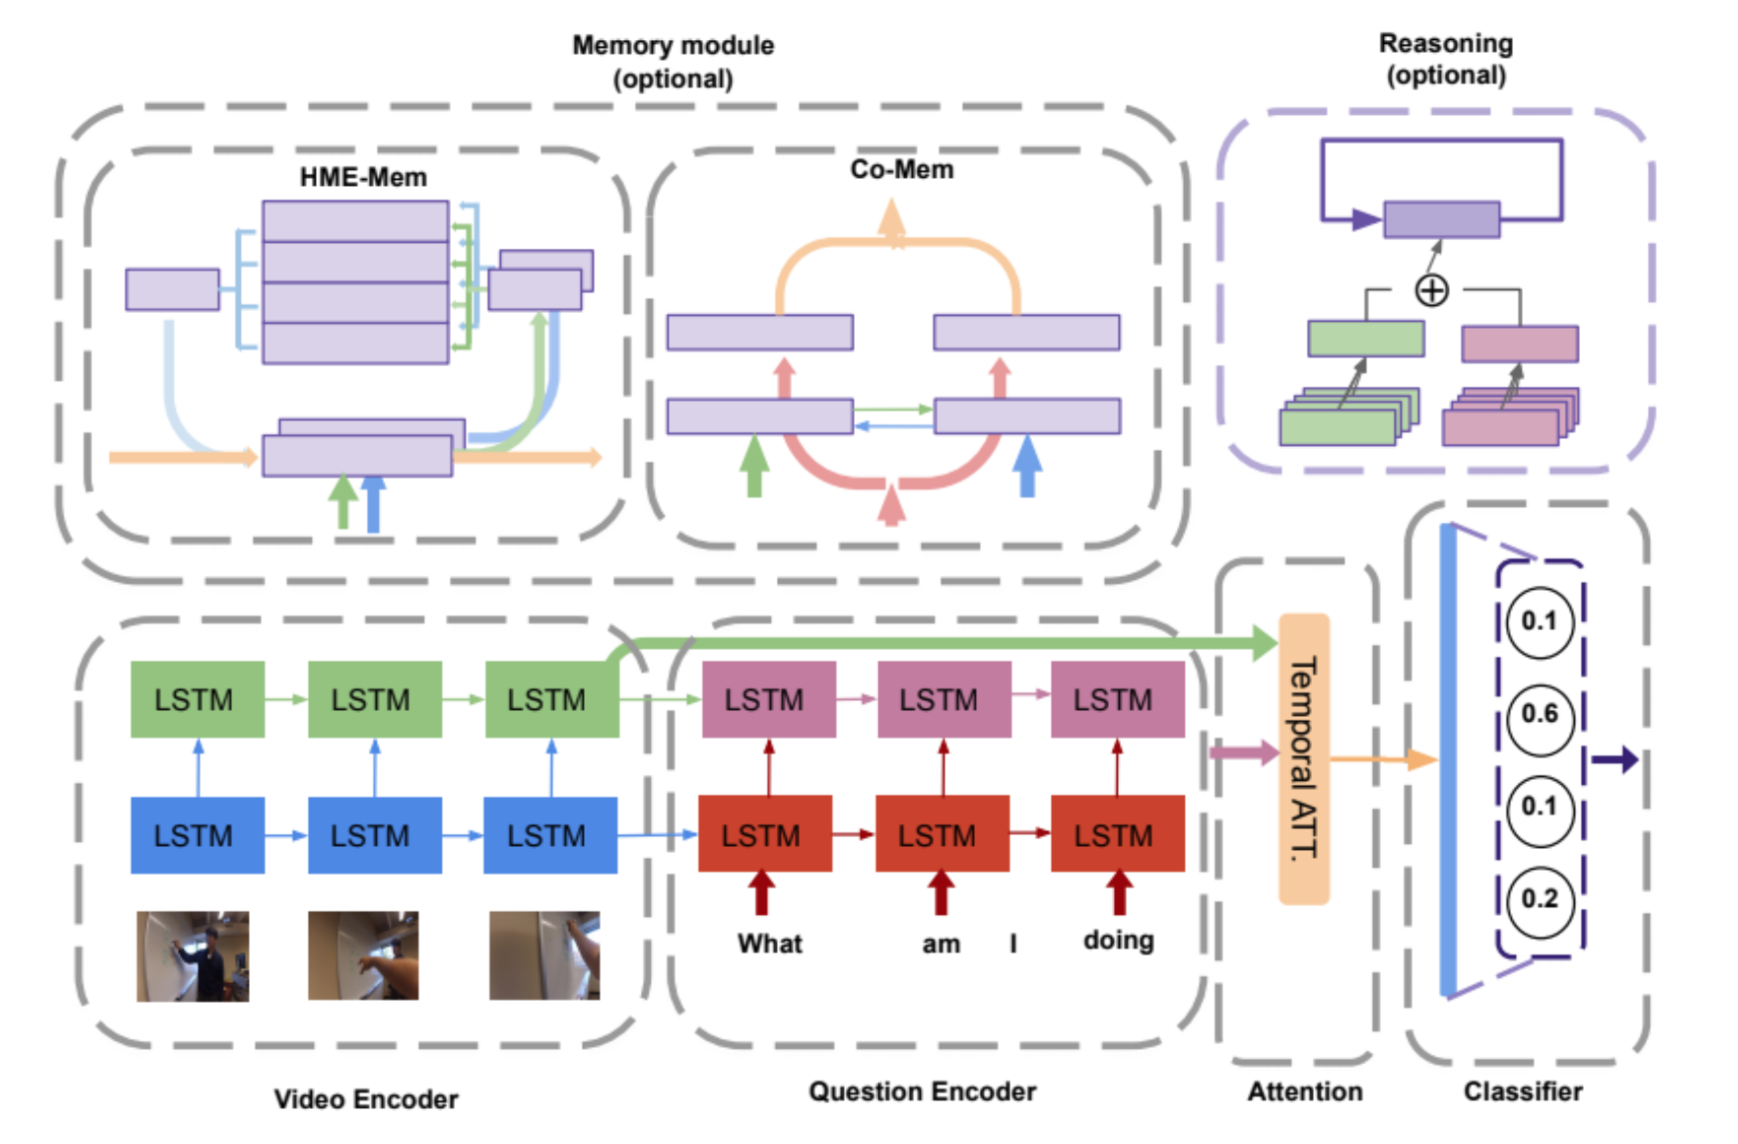
\includegraphics[width=0.9\textwidth]{video-qa-arch.png}
  \caption{Typical VideoQA architecture. Figure from~\cite{dataset:ego-vqa}.}
  \label{fig:video-qa-arch}
\end{figure}


\subsection{External Knowledge for VQA}

While VideoQA research has focused on end-to-end neural network architectures, some recent research in VQA (single frame setting) has experimented with using explicit reasoning layers and integrating external knowledge. A number of VQA datasets which require some form of external `commonsense' reasoning have been proposed recently~\cite{dataset:ok-vqa, dataset:fvqa, dataset:kb-vqa}. It has been shown that end-to-end neural networks which do not attempt to make use of knowledge which is external to the training data perform poorly on some of these datasets~\cite{dataset:ok-vqa}. This section discusses some of the attempts that have been made to integrate external knowledge into VQA systems.

The authors of the three datasets outlined above propose models which make use of external knowledge, ususally stored in some structured knowledge base (KB), such as DBpedia~\cite{kb:dbpedia}, which stores structured information extracted from Wikipedia, or ConceptNet~\cite{kb:conceptnet}, which contains automatically generated `commonsense' relations between objects.

As opposed to using a structured KB, the authors of~\cite{dataset:ok-vqa} provide a neural network model which is trained to find the answer to an image-question pair from Wikipedia articles. They also propose a number of methods for combining this network with state-of-the-art VQA models and show that this provides an improvement in performance on their dataset.

The authors of~\cite{explicit-reasoning-vqa} propose a model which first extracts properties from an image using a pre-trained neural network and represents these properties explicitly using logic. They also extract relations between nouns, adjectives and the question word from the question and represent these in logic. Finally, they reason over the extracted relations using a probabilistic reasoning engine to find the most likely answer. This method of reasoning not only allows the model to make use of external knowledge, but also helps improve the transparency and explainability of the model.


\end{document}
